\section{Einleitung}
\label{sec:Einleitung}

In diesem Versuch werden verschiedene Metallestäbe erwärmt und die Temperatur an unterschiedlichen Punkten gemessen.
Ziel ist es, aus den Temperaturverläufen anschließend die Wärmeleitfähigkeit der Metalle zu bestimmen. 

\section{Theorie}
\label{sec:Theorie}

\subsection{Wärmeleitung und Wärmeleitfähigkeit}
\label{sec:Wärmeleitung und Wärmeleitfähigkeit}

Befindet sich ein Körper nicht im Temperaturgleichgewicht, so wird die Wärme entlang des Temperaturgefälles durch
den Körper transportiert. Die Wärme bewegt sich dabei immer in Richtung der kälteren Temperatur.

Betrachtet man wie in diesem Versuch Stäbe mit der Querschnittsfläche $A$ aus einem Material mit der Dichte $\rho$, 
spezifischen Wärme $c$ und der Wärmeleitfähigkeit $\kappa$, dann fließt in der Zeit $dt$ die Wärmemenge

\begin{equation}
    dQ = -\kappa A\frac{\partial T}{\partial x}dt
    \label{eq:Wärmemenge}
\end{equation}

durch die Querschnittsfläche des Stabes. \cite{v204}

Wenn der Stab nun abwechselnd mit der Periode $T$ erwärmt und gekühlt wird, dann lässt sich die Wärmeleitfähigkeit
$\kappa$ aus den Eigenschaften der Temperaturwelle berechnen.
Misst man zwei Temperaturamplituden $A_{\symup{nah}}$ und $A_{\symup{fern}}$ an zwei Messstellen mit dem Abstand $\symup{\Delta} x$
sowie die zugehörige Phasendifferenz $\symup{\Delta} t$ der Temperaturwelle dann gilt

\begin{equation}
    \kappa =\frac{\rho c(\symup{\Delta} x)^{2}}{2\symup{\Delta} t\,\textup{ln}(\frac{A_{\symup{nah}}}{A_{\symup{fern}}})}.
    \label{eq:Kappa}
\end{equation}

für jedes beliebige Messwertepaar $x_{\symup{nah}}$ und $x_{\symup{fern}}$. \cite{v204}

\subsection{Versuchsaufbau}
\label{sec:Versuchsaufbau}

Der Aufbau des Experiementes ist in \autoref{fig:Versuchsaufbau} dargestellt.
Auf einer Grundplatte befinden sich vier Metallestäbe, die mit einem Peltierelement geheizt bzw. gekühlt werden können.
Zwei der Stäbe bestehen aus Messing mit unterschiedlichen Querschnittsflächen $A$, das Material der anderen Stäbe ist
Aluminium bzw. Edelstahl.

Bei jedem Stab lässt sich die Temperatur an zwei Stellen messen, somit werden insgesamt acht Temperaturwerte ($T_{1}$ bis $T_{8}$) je
Zeitpunkt aufgenommen und digital mit dem \glqq Xplorer GLX\grqq{} erfasst.

\begin{figure} [H]
    \centering
    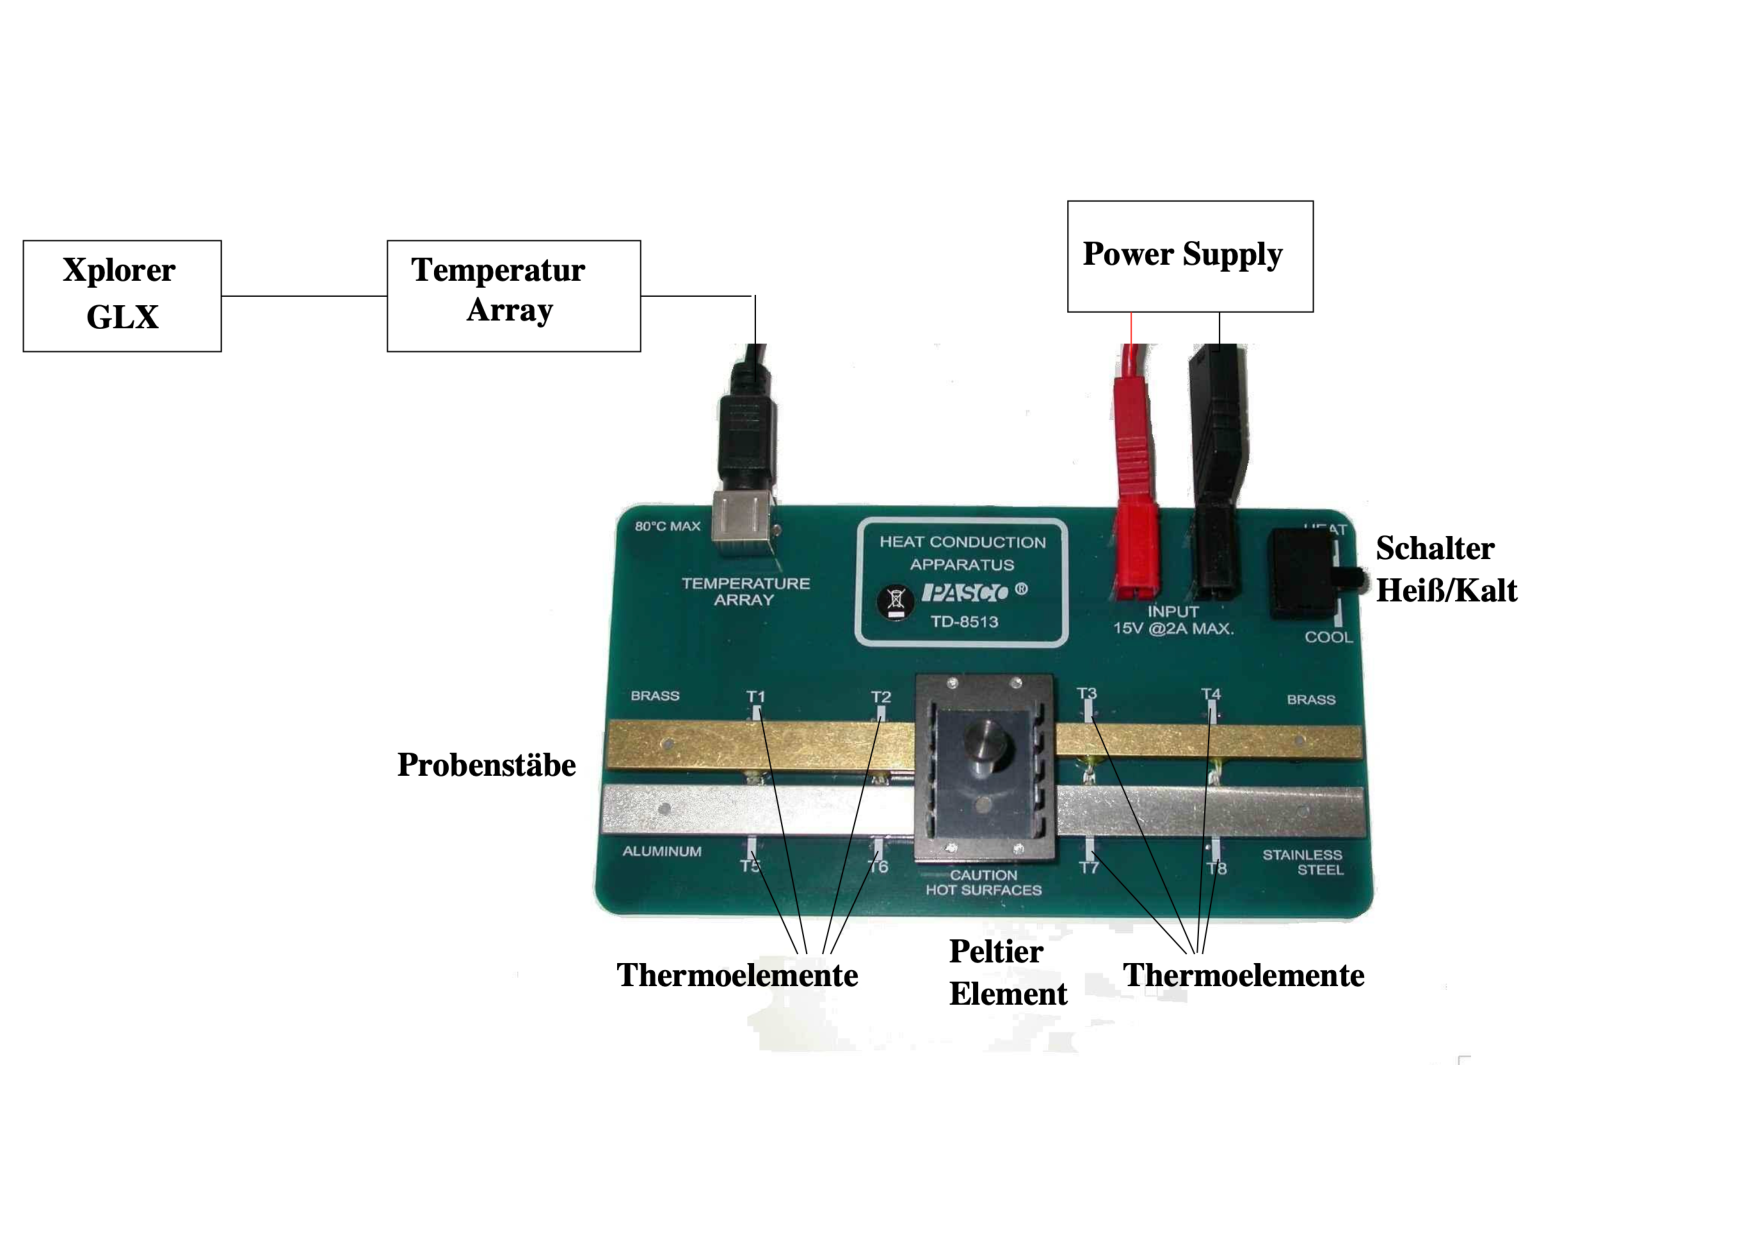
\includegraphics[height=10cm]{content/Abbildungen/Versuchsaufbau.pdf}
    \caption{Grundplatte mit vier Probestäben und Heizelement.\cite{v204}}
    \label{fig:Versuchsaufbau}
\end{figure}